% When a window fires and what the latency experiment measures (run_latency.sh, analyze.py).
% Schematic: distances are not to scale.
\documentclass[tikz,border=4pt]{standalone}
\usepackage[T1]{fontenc}
\usepackage{lmodern}
\usetikzlibrary{positioning,arrows.meta,calc,decorations.pathreplacing}
% Shared look for every diagram. \input this after \usetikzlibrary.
% Greys plus one accent, so the figures print fine in black and white.
\definecolor{accent}{HTML}{2563EB}
\definecolor{accentlight}{HTML}{DBEAFE}
\definecolor{latecol}{HTML}{B45309}
\definecolor{latelight}{HTML}{FEF3C7}
\definecolor{grey}{HTML}{6B7280}
\definecolor{greylight}{HTML}{F3F4F6}
\tikzset{
  box/.style={draw, rounded corners=2pt, align=center, minimum height=7mm, inner sep=3pt, fill=white, font=\footnotesize},
  topic/.style={box, fill=greylight, draw=grey},
  op/.style={box, draw=accent, fill=accentlight},
  ctr/.style={draw=grey, dashed, rounded corners=4pt, inner sep=3mm},
  note/.style={font=\scriptsize, text=grey, align=left},
  arr/.style={-{Latex[length=2mm]}, thick},
  shuffle/.style={arr, double, double distance=0.6pt, -{Latex[length=2.4mm]}},
  latearr/.style={arr, dashed, draw=latecol},
  lbl/.style={font=\scriptsize, fill=white, inner sep=1pt},
}

\begin{document}
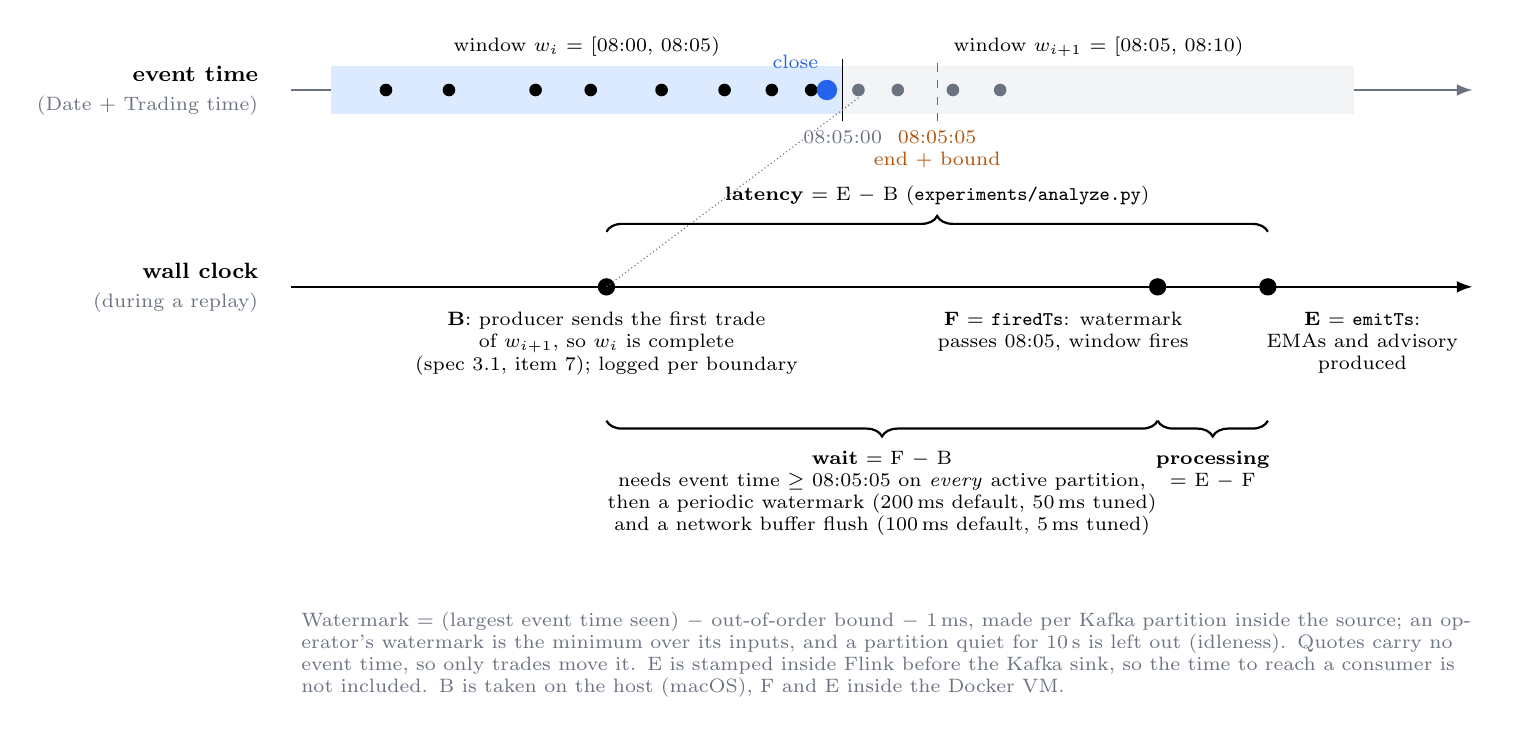
\begin{tikzpicture}[x=1mm,y=1mm]
  % ---------------- lane 1: event time
  \node[font=\footnotesize\bfseries, anchor=east] at (-3,30) {event time};
  \node[note, anchor=east] at (-3,26) {(Date + Trading time)};
  \draw[arr, draw=grey] (0,28) -- (150,28);
  \fill[accentlight] (5,25) rectangle (70,31);
  \fill[greylight] (70,25) rectangle (135,31);
  \node[font=\scriptsize] at (37.5,33.5) {window $w_i$ = [08:00, 08:05)};
  \node[font=\scriptsize] at (102.5,33.5) {window $w_{i+1}$ = [08:05, 08:10)};
  \draw (70,24) -- (70,32);
  \node[note, below] at (70,24) {08:05:00};
  \draw[dashed, draw=latecol] (82,24) -- (82,32);
  \node[note, below, text=latecol, align=center] at (82,24) {08:05:05\\end + bound};
  % trades of w_i, last one is the close
  \foreach \x in {12,20,31,38,47,55,61,66} \fill (\x,28) circle (0.8);
  \fill[accent] (68,28) circle (1.3);
  \node[font=\scriptsize, text=accent, anchor=south] at (64,29.5) {close};
  \foreach \x in {72,77,84,90} \fill[grey] (\x,28) circle (0.8);

  % ---------------- lane 2: wall clock
  \node[font=\footnotesize\bfseries, anchor=east] at (-3,5) {wall clock};
  \node[note, anchor=east] at (-3,1) {(during a replay)};
  \draw[arr] (0,3) -- (150,3);
  \coordinate (B) at (40,3); \coordinate (F) at (110,3); \coordinate (E) at (124,3);
  \foreach \p/\t/\s in {B/{\textbf{B}: producer sends the first trade\\of $w_{i+1}$ ($w_i$ is now complete,\\spec 3.1 item 7); logged per boundary}/below,
                       F/{\textbf{F} = \texttt{firedTs}: watermark\\passes 08:05, window\\fires, close goes on}/below,
                       E/{\textbf{E} = \texttt{emitTs}: EMAs and\\advisory produced in\\\texttt{EmaProcessor}}/above}
    { \fill (\p) circle (1.1); }
  \node[font=\scriptsize, align=center, anchor=north] at ($(B)+(0,-2)$) {\textbf{B}: producer sends the first trade\\of $w_{i+1}$, so $w_i$ is complete\\(spec 3.1, item 7); logged per boundary};
  \node[font=\scriptsize, align=center, anchor=north] at ($(F)+(-12,-2)$) {\textbf{F} = \texttt{firedTs}: watermark\\passes 08:05, window fires};
  \node[font=\scriptsize, align=center, anchor=north] at ($(E)+(12,-2)$) {\textbf{E} = \texttt{emitTs}:\\EMAs and advisory\\produced};
  % mapping first trade of w_{i+1} down to B
  \draw[densely dotted, draw=grey] (72,27) -- (B);
  % braces
  \draw[decorate, decoration={brace, amplitude=2mm, mirror}, thick] ($(B)+(0,-17)$) -- node[below=2.5mm, font=\scriptsize, align=center]{\textbf{wait} = F $-$ B\\needs event time $\ge$ 08:05:05 on \emph{every} active partition,\\then a periodic watermark (200\,ms default, 50\,ms tuned)\\and a network buffer flush (100\,ms default, 5\,ms tuned)} ($(F)+(0,-17)$);
  \draw[decorate, decoration={brace, amplitude=2mm, mirror}, thick] ($(F)+(0,-17)$) -- node[below=2.5mm, font=\scriptsize, align=center]{\textbf{processing}\\= E $-$ F} ($(E)+(0,-17)$);
  \draw[decorate, decoration={brace, amplitude=2mm}, thick] ($(B)+(0,7)$) -- node[above=2mm, font=\scriptsize]{\textbf{latency} = E $-$ B (\texttt{experiments/analyze.py})} ($(E)+(0,7)$);
  \node[note, anchor=north west, text width=150mm] at (0,-37) {Watermark = (largest event time seen) $-$ out-of-order bound $-$ 1\,ms, made per Kafka partition inside the source; an operator's watermark is the minimum over its inputs, and a partition quiet for 10\,s is left out (idleness). Quotes carry no event time, so only trades move it. E is stamped inside Flink before the Kafka sink, so the time to reach a consumer is not included. B is taken on the host (macOS), F and E inside the Docker VM.};
\end{tikzpicture}
\end{document}
